\documentclass[tikz,border=2pt]{standalone}
\usepackage{newpxtext,newpxmath}
\definecolor{curve}{HTML}{1f6fb2}
\definecolor{accent}{HTML}{c0392b}
\definecolor{polygon}{HTML}{555555}
\definecolor{muted}{HTML}{dfe6ee}
\begin{document}
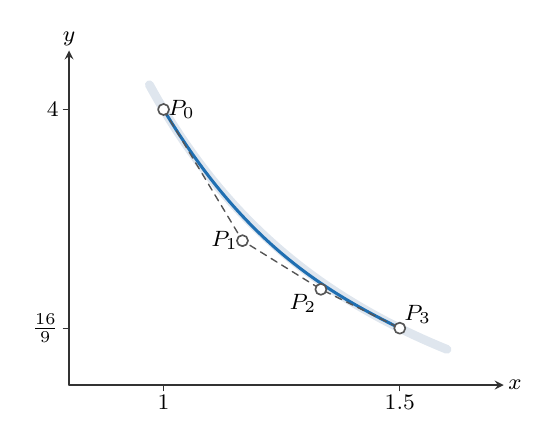
\begin{tikzpicture}[
  x=6cm, y=1.25cm,
  line cap=round, line join=round,
  every node/.style={font=\footnotesize, inner sep=1.5pt},
  curve/.style={draw=curve, line width=1.1pt},
  second/.style={draw=accent, line width=1.1pt},
  polygon/.style={line width=0.5pt, dash pattern=on 2.5pt off 2pt},
  construction/.style={draw=accent, line width=0.5pt},
  axis/.style={line width=0.45pt, draw=black!80, >=stealth},
  ctrl/.style={circle, fill=white, line width=0.6pt, minimum size=4pt, inner sep=0pt},
]
\draw[axis, ->] (0.8,1.2) -- (1.72,1.2) node[right] {$x$};
\draw[axis, ->] (0.8,1.2) -- (0.8,4.6) node[above] {$y$};
\draw[axis] (1,1.2) -- ++(0,-2pt) node[below] {$1$};
\draw[axis] (1.5,1.2) -- ++(0,-2pt) node[below] {$1.5$};
\draw[axis] (0.8,4) -- ++(-2pt,0) node[left] {$4$};
\draw[axis] (0.8,1.778) -- ++(-2pt,0) node[left] {$\frac{16}{9}$};
\draw[draw=muted, line width=3.2pt] (0.9700,4.2512) .. controls (0.9962,4.0212) and (1.0225,3.8188) .. (1.0488,3.6368) .. controls (1.0750,3.4547) and (1.1013,3.2930) .. (1.1275,3.1465) .. controls (1.1538,3.0000) and (1.1800,2.8687) .. (1.2063,2.7491) .. controls (1.2325,2.6294) and (1.2588,2.5214) .. (1.2850,2.4224) .. controls (1.3113,2.3235) and (1.3375,2.2335) .. (1.3638,2.1508) .. controls (1.3900,2.0680) and (1.4163,1.9923) .. (1.4425,1.9223) .. controls (1.4950,1.7824) and (1.5475,1.6650) .. (1.6000,1.5625);
\draw[curve] (1.0000,4.0000) .. controls (1.1667,2.6667) and (1.3333,2.1728) .. (1.5000,1.7778);
\draw[polygon, draw=polygon] (1,4) -- (1.167,2.667) -- (1.333,2.173) -- (1.5,1.778);
\node[ctrl, draw=polygon] at (1,4) {};
\node[ctrl, draw=polygon] at (1.167,2.667) {};
\node[ctrl, draw=polygon] at (1.333,2.173) {};
\node[ctrl, draw=polygon] at (1.5,1.778) {};
\node[right] at (1,4) {$P_0$};
\node[left] at (1.167,2.667) {$P_1$};
\node[below left] at (1.333,2.173) {$P_2$};
\node[above right] at (1.5,1.778) {$P_3$};
\end{tikzpicture}
\end{document}
